\documentclass[twoside]{book}

% Packages required by doxygen
\usepackage{fixltx2e}
\usepackage{calc}
\usepackage{doxygen}
\usepackage{graphicx}
\usepackage[utf8]{inputenc}
\usepackage{makeidx}
\usepackage{multicol}
\usepackage{multirow}
\PassOptionsToPackage{warn}{textcomp}
\usepackage{textcomp}
\usepackage[nointegrals]{wasysym}
\usepackage[table]{xcolor}

% Font selection
\usepackage[T1]{fontenc}
\usepackage{mathptmx}
\usepackage[scaled=.90]{helvet}
\usepackage{courier}
\usepackage{amssymb}
\usepackage{sectsty}
\renewcommand{\familydefault}{\sfdefault}
\allsectionsfont{%
  \fontseries{bc}\selectfont%
  \color{darkgray}%
}
\renewcommand{\DoxyLabelFont}{%
  \fontseries{bc}\selectfont%
  \color{darkgray}%
}
\newcommand{\+}{\discretionary{\mbox{\scriptsize$\hookleftarrow$}}{}{}}

% Page & text layout
\usepackage{geometry}
\geometry{%
  a4paper,%
  top=2.5cm,%
  bottom=2.5cm,%
  left=2.5cm,%
  right=2.5cm%
}
\tolerance=750
\hfuzz=15pt
\hbadness=750
\setlength{\emergencystretch}{15pt}
\setlength{\parindent}{0cm}
\setlength{\parskip}{0.2cm}
\makeatletter
\renewcommand{\paragraph}{%
  \@startsection{paragraph}{4}{0ex}{-1.0ex}{1.0ex}{%
    \normalfont\normalsize\bfseries\SS@parafont%
  }%
}
\renewcommand{\subparagraph}{%
  \@startsection{subparagraph}{5}{0ex}{-1.0ex}{1.0ex}{%
    \normalfont\normalsize\bfseries\SS@subparafont%
  }%
}
\makeatother

% Headers & footers
\usepackage{fancyhdr}
\pagestyle{fancyplain}
\fancyhead[LE]{\fancyplain{}{\bfseries\thepage}}
\fancyhead[CE]{\fancyplain{}{}}
\fancyhead[RE]{\fancyplain{}{\bfseries\leftmark}}
\fancyhead[LO]{\fancyplain{}{\bfseries\rightmark}}
\fancyhead[CO]{\fancyplain{}{}}
\fancyhead[RO]{\fancyplain{}{\bfseries\thepage}}
\fancyfoot[LE]{\fancyplain{}{}}
\fancyfoot[CE]{\fancyplain{}{}}
\fancyfoot[RE]{\fancyplain{}{\bfseries\scriptsize 2014年12月24日(水) 15時50分58秒作成 -\/ Log / 構成\+:  Doxygen }}
\fancyfoot[LO]{\fancyplain{}{\bfseries\scriptsize 2014年12月24日(水) 15時50分58秒作成 -\/ Log / 構成\+:  Doxygen }}
\fancyfoot[CO]{\fancyplain{}{}}
\fancyfoot[RO]{\fancyplain{}{}}
\renewcommand{\footrulewidth}{0.4pt}
\renewcommand{\chaptermark}[1]{%
  \markboth{#1}{}%
}
\renewcommand{\sectionmark}[1]{%
  \markright{\thesection\ #1}%
}

% Indices & bibliography
\usepackage{natbib}
\usepackage[titles]{tocloft}
\setcounter{tocdepth}{3}
\setcounter{secnumdepth}{5}
\makeindex

% Hyperlinks (required, but should be loaded last)
\usepackage{ifpdf}
\ifpdf
  \usepackage[pdftex,pagebackref=true]{hyperref}
\else
  \usepackage[ps2pdf,pagebackref=true]{hyperref}
\fi
\hypersetup{%
  colorlinks=true,%
  linkcolor=blue,%
  citecolor=blue,%
  unicode%
}

% Custom commands
\newcommand{\clearemptydoublepage}{%
  \newpage{\pagestyle{empty}\cleardoublepage}%
}


%===== C O N T E N T S =====

\begin{document}

% Titlepage & ToC
\hypersetup{pageanchor=false,
             bookmarks=true,
             bookmarksnumbered=true,
             pdfencoding=unicode
            }
\pagenumbering{roman}
\begin{titlepage}
\vspace*{7cm}
\begin{center}%
{\Large Log }\\
\vspace*{1cm}
{\large 構築\+: Doxygen 1.8.8}\\
\vspace*{0.5cm}
{\small 2014年12月24日(水) 15時50分58秒}\\
\end{center}
\end{titlepage}
\clearemptydoublepage
\tableofcontents
\clearemptydoublepage
\pagenumbering{arabic}
\hypersetup{pageanchor=true}

%--- Begin generated contents ---
\chapter{階層索引}
\section{クラス階層}
クラス階層一覧です。大雑把に文字符号順で並べられています。\begin{DoxyCompactList}
\item Exception\begin{DoxyCompactList}
\item \contentsline{section}{Log\+Exception}{\pageref{class_log_exception}}{}
\end{DoxyCompactList}
\item \contentsline{section}{Log}{\pageref{class_log}}{}
\end{DoxyCompactList}

\chapter{データ構造索引}
\section{データ構造}
データ構造一覧です。\begin{DoxyCompactList}
\item\contentsline{section}{\hyperlink{class_log}{Log} }{\pageref{class_log}}{}
\item\contentsline{section}{\hyperlink{class_log_exception}{Log\+Exception} }{\pageref{class_log_exception}}{}
\end{DoxyCompactList}

\chapter{データ構造詳解}
\hypertarget{class_log}{\section{Log クラス}
\label{class_log}\index{Log@{Log}}
}
\subsection*{公開メンバ関数}
\begin{DoxyCompactItemize}
\item 
\hyperlink{class_log_a67b87fd77dbcba71a2cc1003242b4025}{\+\_\+\+\_\+construct} (\$log\+Nm= 'error.\+log', \$log\+Dir= '.', \$is\+Ym\+Div=T\+R\+U\+E, \$is\+Err\+Disp=T\+R\+U\+E)
\item 
\hyperlink{class_log_aa757d15952223c276bf6355dd20a4c65}{out} ()
\item 
\hyperlink{class_log_a982b6a779ab20914da936c96363ffac3}{get\+Log\+Nm} ()
\item 
\hyperlink{class_log_adf01d6c05e9e80681754d2a9f2bb4cba}{get\+Log\+Full\+Path} ()
\item 
\hyperlink{class_log_ade71d11396892967682c9dc03049a0f3}{get\+Log\+Dir\+Path} ()
\end{DoxyCompactItemize}


\subsection{詳解}
ログクラス

\begin{DoxyVersion}{バージョン}
1.\+1.\+1  U\+T\+F-\/8  2011/02/15  2014/12/24  M\+I\+T 
\end{DoxyVersion}
\begin{DoxyAuthor}{著者}
mamiya\+\_\+shou 
\end{DoxyAuthor}
\begin{DoxyCopyright}{著作権所有}
mamiya\+\_\+shou  P\+H\+P 5.\+0 以上必須 
\end{DoxyCopyright}


\subsection{構築子と解体子}
\hypertarget{class_log_a67b87fd77dbcba71a2cc1003242b4025}{\index{Log@{Log}!\+\_\+\+\_\+construct@{\+\_\+\+\_\+construct}}
\index{\+\_\+\+\_\+construct@{\+\_\+\+\_\+construct}!Log@{Log}}
\subsubsection[{\+\_\+\+\_\+construct}]{\setlength{\rightskip}{0pt plus 5cm}\+\_\+\+\_\+construct (
\begin{DoxyParamCaption}
\item[{}]{\$log\+Nm = {\ttfamily 'error.log'}, }
\item[{}]{\$log\+Dir = {\ttfamily '.'}, }
\item[{}]{\$is\+Ym\+Div = {\ttfamily TRUE}, }
\item[{}]{\$is\+Err\+Disp = {\ttfamily TRUE}}
\end{DoxyParamCaption}
)}}\label{class_log_a67b87fd77dbcba71a2cc1003242b4025}
エラー時にメッセージを表示するかどうか コンストラクタ


\begin{DoxyParams}[1]{引数}
string & {\em \$log\+Nm} & ログファイル名 (def\+:'error.\+log') \\
\hline
string & {\em \$log\+Dir} & ログファイルのディレクトリ (def\+:'.') \\
\hline
boolean & {\em \$is\+Ym\+Div} & ログファイル名に年月を追加してファイル分けるかどうか (def\+:T\+R\+U\+E) \\
\hline
boolean & {\em \$is\+Err\+Disp} & エラー時にメッセージを表示するかどうか (def\+:T\+R\+U\+E) \\
\hline
\end{DoxyParams}


\subsection{関数詳解}
\hypertarget{class_log_ade71d11396892967682c9dc03049a0f3}{\index{Log@{Log}!get\+Log\+Dir\+Path@{get\+Log\+Dir\+Path}}
\index{get\+Log\+Dir\+Path@{get\+Log\+Dir\+Path}!Log@{Log}}
\subsubsection[{get\+Log\+Dir\+Path}]{\setlength{\rightskip}{0pt plus 5cm}get\+Log\+Dir\+Path (
\begin{DoxyParamCaption}
{}
\end{DoxyParamCaption}
)}}\label{class_log_ade71d11396892967682c9dc03049a0f3}
ログディレクトリのパスを返す

\begin{DoxyReturn}{戻り値}
string ログディレクトリのパス 
\end{DoxyReturn}
\hypertarget{class_log_adf01d6c05e9e80681754d2a9f2bb4cba}{\index{Log@{Log}!get\+Log\+Full\+Path@{get\+Log\+Full\+Path}}
\index{get\+Log\+Full\+Path@{get\+Log\+Full\+Path}!Log@{Log}}
\subsubsection[{get\+Log\+Full\+Path}]{\setlength{\rightskip}{0pt plus 5cm}get\+Log\+Full\+Path (
\begin{DoxyParamCaption}
{}
\end{DoxyParamCaption}
)}}\label{class_log_adf01d6c05e9e80681754d2a9f2bb4cba}
ログファイルのフルパスを返す

\begin{DoxyReturn}{戻り値}
string ログファイルのフルパス 
\end{DoxyReturn}
\hypertarget{class_log_a982b6a779ab20914da936c96363ffac3}{\index{Log@{Log}!get\+Log\+Nm@{get\+Log\+Nm}}
\index{get\+Log\+Nm@{get\+Log\+Nm}!Log@{Log}}
\subsubsection[{get\+Log\+Nm}]{\setlength{\rightskip}{0pt plus 5cm}get\+Log\+Nm (
\begin{DoxyParamCaption}
{}
\end{DoxyParamCaption}
)}}\label{class_log_a982b6a779ab20914da936c96363ffac3}
ログファイル名を返す

\begin{DoxyReturn}{戻り値}
string ログファイルのフルパス 
\end{DoxyReturn}
\hypertarget{class_log_aa757d15952223c276bf6355dd20a4c65}{\index{Log@{Log}!out@{out}}
\index{out@{out}!Log@{Log}}
\subsubsection[{out}]{\setlength{\rightskip}{0pt plus 5cm}out (
\begin{DoxyParamCaption}
{}
\end{DoxyParamCaption}
)}}\label{class_log_aa757d15952223c276bf6355dd20a4c65}
ログファイルに書き込む

\begin{DoxyReturn}{戻り値}
boolean 書き込みの成否  引数に指定されたモノをカンマで結合し出力 
\end{DoxyReturn}


このクラス詳解は次のファイルから抽出されました\+:\begin{DoxyCompactItemize}
\item 
Log/Log.\+php\end{DoxyCompactItemize}

\hypertarget{class_log_exception}{\section{Log\+Exception クラス}
\label{class_log_exception}\index{Log\+Exception@{Log\+Exception}}
}
Log\+Exception の継承関係図\begin{figure}[H]
\begin{center}
\leavevmode
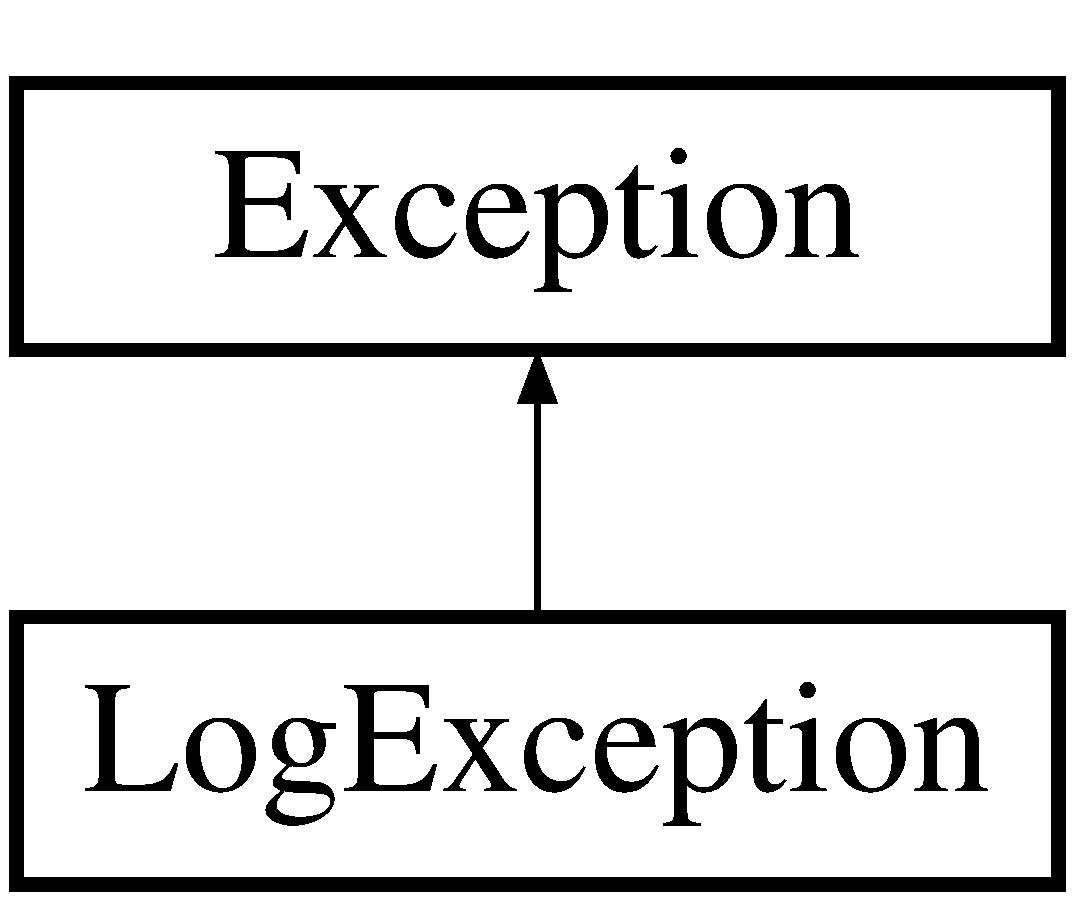
\includegraphics[height=2.000000cm]{class_log_exception}
\end{center}
\end{figure}


\subsection{詳解}
Log\+Exceptionクラス

Exceptionクラスを継承 

このクラス詳解は次のファイルから抽出されました\+:\begin{DoxyCompactItemize}
\item 
Log/Log.\+php\end{DoxyCompactItemize}

%--- End generated contents ---

% Index
\newpage
\phantomsection
\addcontentsline{toc}{chapter}{索引}
\printindex

\end{document}
